\chapter{Parallelisierung der kritischen Abschnitte}

Um der optimalen Leistung nah zu kommen, wurde bei der Implementierung ein iterativer Ansatz gewählt. Hierzu wurden zuerst die Möglichkeiten der Parallelisierung und anschließend die, der Optimierung in Python betrachtet. 

\section{Parallelisierung}

\subsection{Parallelisierung der Verarbeitung einzelner Bildpaare mittels MPI}

Da die zu bearbeitenden Bildpaare voneinander unabhängig sind, lassen diese sich trivial parallelisieren. Der Vorteil dieses Ansatzes liegt besonders in seiner simplen Implementierung und erwarteten linearen Skalierung begründet. Dieser Ansatz bringt allerdings auch einige Nachteile mit sich: Einige \gls{MPI}-Implementierungen erlauben das Erstellen neuer Threads nur, wenn dies beim Installieren der Bibliotheken angegeben wird\footnote{\url{https://www.open-mpi.org/doc/v2.0/man3/MPI_Init_thread.3.php}} und es ist nur eine schwache Skalierung zu erwarten. Sofern kein Multithreading innerhalb von \gls{MPI} möglich ist, limitiert die Anzahl der Bildpaare die Parallelisierungsmöglichkeit stark. Die Implementierung dieses Ansatzes ist auf dem GitHub-Branch \textit{mpi}\footnote{\url{https://github.com/ComputationalRadiationPhysics/Wavefront-Sensor/tree/551403ef16024e2ab53e50e3c0ed3619683e3fcf}} verfügbar.

\subsection{Parallelisierung innerhalb der Verarbeitung einzelner Bildpaare mittels MPI}

Eine sinnvolle Erweiterung zur oben beschriebenen Methode ist das Ersetzen der genutzten Mul\-ti\-threa\-ding-Bibliothek mittels MPI, sodass selbst die Berechnung eines einzelnen Bildpaares über Rechnergrenzen hinweg möglich ist. In diesem Zuge wurde auch die Fehlerkorrektur am Ende des Speckle-Trackings parallelisiert, indem die zu korrigierende Bildausschnitte auf mehrere Kerne verteilt wurden. Zusätzlich ermöglicht diese Implementierung den Einsatz eines Tracing-Programmes, wie SCORE-P\footnote{\url{http://www.vi-hps.org/projects/score-p/}}. Dies war aufgrund der unterliegenden multiprocessing-Bibliothek zuvor nicht möglich. Ein hoher Speedup wird insbesondere für wenige zu korrigierende Bildausschnitte nicht erwartet. 

Im Konkreten werden die Bildpaare auf \gls{CPU}-Kern Gruppen verteilt. Einer dieser Kerne innerhalb der Gruppe agiert hierbei als Hauptkern und ist dafür verantwortlich das Bildpaar zu verarbeiten, wobei dieser Aufgaben mittels eines \gls{MPI}-Kommunikators an die anderen Rechenkerne der Gruppe verteilen kann. Die Aufgabe des Wurzelkerns ist es, die Bildpaare gleichmäßig auf die Gruppen zu verteilen. Dies ist in der Abbildung \ref{fig:parallel_concept} gezeigt. Die Schnittstelle wurde hierbei ähnlich zur joblib-Implementierung entworfen. Sollten mehr Bildpaare als Rechenkerne vorhanden sein, werden mehrere Bildpaare von eine Kern hintereinander verarbeitet. Die Programmierschnittstelle wurde so entworfen, dass die Verteilung der Bildpaare auf die Kernen und das Parallelisieren innerhalb dieser für den Programmierer transparent geschieht. Die Implementierung dieses Ansatzes ist auf GitHub auf dem \textit{mpi-advanced}-Branch\footnote{\url{https://github.com/ComputationalRadiationPhysics/Wavefront-Sensor/tree/773ee2d4006c71c2b7acacf33931a7a1356255ee}} zu finden.

\begin{center}
	\begin{figure}[htbp]
		\centering
		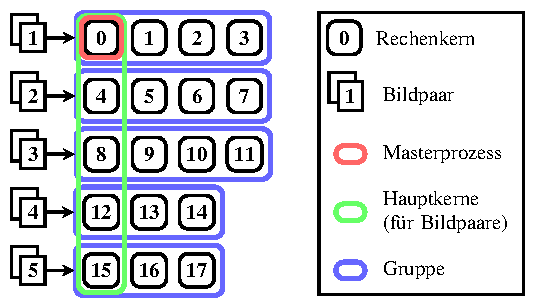
\includegraphics[width=0.5\textwidth]{pdf/parallel}
		\caption[Verteilung]{Verteilung von fünf Bildpaaren auf 18 Rechenknoten}
		\label{fig:parallel_concept}
	\end{figure}
\end{center}

\section{Optimierung der Python-Engpässe}

Wie in Abbildung \ref{fig:perc_slow} zu sehen ist, wird über 95\% der Rechenzeit in den fünf langsamsten Funktionen verbracht. Unter diesen ist insbesondere die \textit{nxcorr\_disp()}-Funktion, welche komplett in Python implementiert ist. Um die Leistung solcher Funktionen zu verbessern werden im folgenden Methoden zur Optimierung des bestehenden Codes betrachtet mit besonderem Augenmerk auf der Optimierung der langsamsten Funktionen. 

\subsection{Nutzen bereits optimierter Funktionen}

Einige Teile des Codes können durch bereits in Python oder einer optimierten Bibliothek enthaltenen Funktion ersetzt werden, womit der Interpretieraufwand erheblich reduziert wird. Dies gehört damit zu einer der grundlegenden Optimierungsmöglichkeiten. Zusätzlich dazu enthalten diese Funktionen bereits Plattform-spezifische Optimierungen. In der Funktion \textit{nxcorr\_disp()} lassen sich Code-Abschnitte mit diesem Verbesserungspotential finden. Das Listing \ref{lst:max2} zeigt den Code aus dieser Funktion zum Ermitteln eines Maximums einer Matrix in reinem Python-Code, wobei die äußeren Zeilen und Spalten vernachlässigt werden. Listing \ref{lst:max2_fast} zeigt einen funktional äquivalenten Code unter Nutzung von bereits optimierten Funktionen. 

\begin{lstlisting}[caption={Finden des Maximums einer Matrix}, label={lst:max2}]
for i in range(1,lengthY-1):
	for j in range(1,lengthX-1):
		if (nxcorr[i, j] > maxValue):
			maxValue = nxcorr[i, j]
			maxI = i
			maxJ = j
\end{lstlisting}

\begin{lstlisting}[caption={Finden des Maximums einer Matrix mittels NumPy und OpenCV}, label={lst:max2_fast}]
nxcorr_small = nxcorr[1:-1,1:-1]
(_, maxValue, _, (maxJ, maxI)) = cv2.minMaxLoc(nxcorr_small)
maxI += 1
maxJ += 1
\end{lstlisting}

Des Weiteren befindet sich in der \textit{nxcorr\_disp()}-Funktion die Berechnung des Signal-Rausch-Verhältnisses (gezeigt im Listing \ref{lst:snr_calc}), was allerdings im weiteren Verlauf des Programmes nicht wieder verwendet wird und deshalb entfernt werden kann. 

\begin{lstlisting}[caption={Berechnung des Signal-Rausch-Verhältnisses}, label={lst:snr_calc}]
avg = 0.0
count = 0
for i in range(lengthY):
	for j in range(lengthX):
		if ((i is not maxI) and (j is not maxJ)):
			avg = avg + abs(nxcorr[i,j])
			count = count + 1
avg = avg / float(count)
SNr = maxValue / avg
\end{lstlisting}

Nach dem Anwenden dieser Änderungen befindet sich keine in Python implementierte Schleife mehr in der Funktion. Angesichts der hohen Aufrufzahl von \textit{nxcorr\_disp()} und dem Entfernen großer Codeanteile ist ein hoher Beschleunigungsfaktor zu erwarten. Die hier angegebenen Verbesserungen sind auf dem Branch \textit{intrinsics} des GitHub-Repositorys\footnote{\url{https://github.com/ComputationalRadiationPhysics/Wavefront-Sensor/tree/30ea08b03cab0bb1ba264941a08badc66d1df548}} zu finden. 

\subsection{Kompilieren}

Eine weitere Möglichkeit der Minimierung des Python-Engpasses ist die Übersetzung des Codes in nativen Maschinencode. Die möglichen Ansätze hierbei reichen von der Übersetzung des gesamten Programmes über die Übersetzung einzelner Funktionen, die in Python dann als Modul geladen werden können, bis hin zur Nutzung eines just-in-time Compilers, welcher annotierte Funktionen bei dessen ersten Aufruf in nativen Maschinencode übersetzt. 

\subsubsection{Gesamtes Programm}

Die einfachste Möglichkeit der Übersetzung ist es, das gesamte Programm in Maschinencode zu übersetzten. Hierzu kann die Bibliothek Cython\footnote{\url{http://cython.org/}} genutzt werden, welche Python-Code in C übersetzt, was anschließend in Maschinencode übersetzt werden kann. Hierzu wurde nur die Datei \textit{waveFront.py} unübersetzt gelassen, da diese keine rechenaufwendigen Funktionen enthält und diese nur aus anderen Dateien, insbesondere der \textit{func.py} aufruft. Die benötigten Installationsdateien sind auch dem GitHub-Branch \textit{compiled}\footnote{\url{https://github.com/ComputationalRadiationPhysics/Wavefront-Sensor/tree/30ea08b03cab0bb1ba264941a08badc66d1df548}} verfügbar. 

\subsubsection{Einzelne Funktionen}

\paragraph{numba}

numba\footnote{\url{https://numba.pydata.org/}} ist eine Optimierungsbibliothek für Python, welche unter anderem die Möglichkeit bietet, Funktionen \gls{JIT} zu übersetzen und CUDA und OpenCL zu nutzen. 

Funktionen können zur \gls{JIT}-Übersetzung mittels der Annotation \texttt{@jit} markiert werden. Sobald während der Ausführung diese Funktion erreicht wird, übersetzt numba den Code in eine Intermediate-Repräsentation, welche anschließend von LLVM weiter in Maschinencode übersetzt wird. Beim nächsten Aufruf wird sofort der Maschinencode verwendet. Ein permanentes Speichern des Übersetzungsergebnisses ist mittels der Annotiation \texttt{@jit(cached = True)} möglich. Auf dem \textit{numba}-Branch\footnote{\url{https://github.com/ComputationalRadiationPhysics/Wavefront-Sensor/tree/9fb7d312f725845d2f4901a31ef0f1dc7558f0b3}} befindet sich eine Version des Codes, in dem diese Annotationen genutzt werden. 

\paragraph{Cython}

Eine weitere weitaus mächtigere Methode zur Übersetzung einzelner Funktionen bietet die Cython-Bibliothek, welche bereits genutzt wurde, um das gesamte Programm zu übersetzen. Diese führt die Möglichkeit der Typisierung ein und lässt die direkte Einbindung von C zu. 

In der auf dem GitHub-Branch \textit{cython}\footnote{\url{https://github.com/ComputationalRadiationPhysics/Wavefront-Sensor/tree/46837cd12c988db8d8c07d84a5dc748594f5f474}} verfügbaren Version wurden Cython genutzt, um die Funktionen \textit{norm\_xcorr()} und \textit{nxcorr\_disp()} zu übersetzen. Hierbei wurden alle Variablen mit Typen versehen und es wurde die von Cython bereitgestellte Schnittstelle zu NumPy genutzt. Zusätzlich wurden ebenfalls Cython-Annotationen verwendet, die NumPy's Grenzfallbehandlung abschalten. Hierbei wurde ein mal die Kompilierung weiterer Funktionen durchgeführt\footnote{\url{https://github.com/ComputationalRadiationPhysics/Wavefront-Sensor/tree/28ebe30e50f607f42450868f1df628070e332c84}} und ein weiteres mal wurde darauf verzichtet. 